\documentclass{article}

\usepackage{fancyhdr}
\usepackage{extramarks}
\usepackage{amsmath}
\usepackage{amsthm}
\usepackage{amsfonts}
\usepackage{tikz}
\usepackage[plain]{algorithm}
\usepackage{algpseudocode}
\usepackage{listings}
\usepackage{xcolor}

\usetikzlibrary{automata,positioning}

\definecolor{codegreen}{rgb}{0,0.6,0}
\definecolor{codegray}{rgb}{0.5,0.5,0.5}
\definecolor{codepurple}{rgb}{0.58,0,0.82}
\definecolor{backcolour}{rgb}{0.95,0.95,0.92}

%
% Basic Document Settings
%

\topmargin=-0.45in
\evensidemargin=0in
\oddsidemargin=0in
\textwidth=6.5in
\textheight=9.0in
\headsep=0.25in

\linespread{1.1}

\pagestyle{fancy}
\lhead{Yousef Alaa Awad}
\chead{\hmwkClass\: \hmwkTitle}
\rhead{\firstxmark}
\lfoot{\lastxmark}
\cfoot{\thepage}

\renewcommand\headrulewidth{0.4pt}
\renewcommand\footrulewidth{0.4pt}

\setlength\parindent{0pt}

%
% Create Problem Sections
%

\setcounter{secnumdepth}{0}
\newcounter{partCounter}
\newcounter{homeworkProblemCounter}
\setcounter{homeworkProblemCounter}{1}

\newcommand{\hmwkTitle}{Homework\ \#3}
\newcommand{\hmwkClass}{Computer Architecture, Section 379}

%
% Title Page
%

\title{
    \vspace{2in}
    \textmd{\textbf{\hmwkClass:\ \hmwkTitle}}\\
    \normalsize\vspace{0.1in}
    \vspace{3in}
}

\author{Yousef Alaa Awad}

% Problems start here
\begin{document}

\maketitle
\pagebreak

\section{1}
\textbf{Given:} Modify the single-cycle datapath (page 3/3) by implementing the instruction ‘SWI’ (store-word-and-increment). Below is the syntax. The instruction below will store the value in \$t0 to memory location at address (\$s0+88). Then, it will increment \$s0 by 4.
\begin{center}
  \textbf{SWI \$t0, 88(\$s0)}
\end{center}
This is the encoding of the instruction above:
\begin{center}
  \begin{tabular}{|c|c|c|c|}
    \hline
    unique & s0 & t0 & 88 \\
    \hline\hline
    opcode (6) & rs (5) & rt (5) & offset (16) \\
    \hline
  \end{tabular}
\end{center}

\subsection{Draw the changes on the datapath diagram and provide the values of all the control signals.}


\section{2}
\textbf{Given:} Modify the single-cycle datapath by implementing the conditional move instruction ‘MOVNZ’ (move-if-not-zero). Below is the syntax. The instruction below will move \$t1 into \$t0 if \$t2!=0. Otherwise, \$t0 will be set to “0”.
\begin{center}
  \textbf{MOVNZ \$t0, \$t1, \$t2}
\end{center}
This is the encoding of the instruction above:
\begin{center}
  \begin{tabular}{|c|c|c|c|c|c|}
    \hline
    unique & t1 & t2 & t0 & 0 & 0 \\
    \hline\hline
    opcode (6) & rs (5) & rt (5) & rd (5) & shamt (5) & funct (6) \\
    \hline
  \end{tabular}
\end{center}

\subsection{A) Draw the changes on the datapath diagram and provide the values of all the control signals.}

\section{3}
\textbf{Given:} Consider a memory system with the following paramaters:
\begin{itemize}
	\item Translation Lookaside Buffer has 512 entries and is 2-way set associative.
	\item 64KByte L1 Data Cache has 128 byte lines and is also 2-way set associative.
	\item Virtual addresses are 64 bits and physical addresses are 32 bits.
	\item 4KB page size.
\end{itemize}


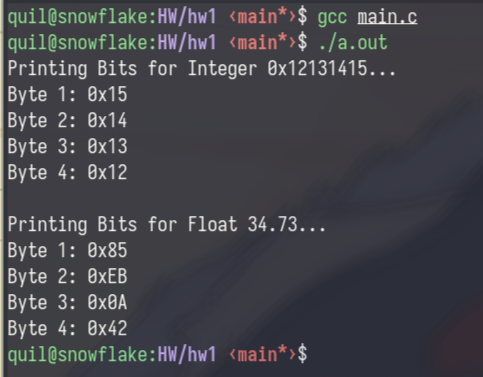
\includegraphics[width=\textwidth]{evidence.png}
\newpage
\lstinputlisting[
	caption=My C Code,
	label={lst:listing-cpp},
	language=C++,
	backgroundcolor=\color{backcolour},   
	commentstyle=\color{codegreen},
	keywordstyle=\color{magenta},
	numberstyle=\tiny\color{codegray},
	stringstyle=\color{codepurple},
	basicstyle=\ttfamily\footnotesize,
	breakatwhitespace=false,         
	breaklines=true,                 
	keepspaces=true,                 
	numbers=left,       
	numbersep=5pt,                  
	showspaces=false,                
	showstringspaces=false,
	showtabs=false,                  
	tabsize=2,
]{main.c}
\newpage

\end{document}
